\chapter{परमाणु के भीतर}\label{ch:g9:inside-the-atom}

1909 में मैनचेस्टर की एक प्रयोगशाला में नन्हे, तेज़ कणों की एक किरणपुंज को
सोने की एक पत्ती पर दाग़ा गया, जो कुछ सौ \omterm{def:g7:atoms-and-molecules:atom}{परमाणु} मोटी थी। लगभग सभी कण सीधे
आर-पार निकल गए, मानो सोना ख़ाली हो। पर कई हज़ार में से लगभग एक कण लौटकर
उछल आया। ``यह ऐसा था मानो तुमने टिशू पेपर के एक टुकड़े पर 15 इंच का गोला
दाग़ा हो और वह लौटकर तुम्हीं से आ टकराया हो,'' अर्नेस्ट रदरफ़ोर्ड ने कहा,
जिनके छात्रों ने यह प्रयोग किया था। \omterm{def:g7:atoms-and-molecules:atom}{परमाणु}, द्रव्य का वह अविभाज्य टुकड़ा, एक
संरचना रखता था --- और वह लगभग पूरी तरह
ख़ाली था।

\begin{recall}
सारा द्रव्य \omterm{def:g7:atoms-and-molecules:atom}{परमाणुओं} से बना है, जिनके लगभग सौ अलग-अलग प्रकार हैं, और हर
प्रकार का \ce{H}, \ce{C}, \ce{O}, \ce{Fe} जैसा एक प्रतीक है। \omterm{def:g7:atoms-and-molecules:atom}{परमाणु} जुड़कर
\omterm{def:g7:atoms-and-molecules:molecule}{अणु} बनाते हैं, जिनका वर्णन \ce{H2O} जैसे सूत्रों से होता है
(\cref{ch:g7:atoms-and-molecules})।
\end{recall}

\section{नाभिक और इलेक्ट्रॉन}

\begin{definition}[नाभिक और इलेक्ट्रॉन]\label{def:g9:inside-the-atom:nucleus}
हर \omterm{def:g7:atoms-and-molecules:atom}{परमाणु} का एक नन्हा, भारी केंद्रीय भाग होता है, \emph{नाभिक}\index{नाभिक},
जिस पर धनात्मक विद्युत आवेश होता है। उसके चारों ओर कहीं हल्के कण घूमते हैं,
\emph{इलेक्ट्रॉन}\index{इलेक्ट्रॉन}, जिनमें से हर एक पर एक ही
ऋणात्मक आवेश, $-e$, होता है।
\end{definition}

\begin{proposition}[परमाणु उदासीन होता है]\label{prop:g9:inside-the-atom:neutral}
% ledger: const:e
पूरे \omterm{def:g7:atoms-and-molecules:atom}{परमाणु} पर कोई विद्युत आवेश नहीं होता: उसके \omterm{def:g9:inside-the-atom:nucleus}{नाभिक} का धनात्मक आवेश
उसके \omterm{def:g9:inside-the-atom:nucleus}{इलेक्ट्रॉनों} के ऋणात्मक आवेशों से ठीक-ठीक संतुलित हो जाता है।
आवेश $e$ बहुत छोटा है: $e = \qty{1.60e-19}{C}$ (आवेश का मात्रक कूलॉम
भौतिकी की पुस्तक का विषय है)।
\end{proposition}

\begin{omfigure}
\begin{tikzpicture}[font=\small]
  \shade[inner color=omDef!35, outer color=white] (0,0) circle (2.2);
  \draw[omDef!60, dashed] (0,0) circle (2.2);
  \foreach \a/\r in {20/1.6,95/1.1,150/1.9,215/1.4,290/1.7,340/0.9} {
    \fill[omDef] (\a:\r) circle (0.06);
    \node[font=\scriptsize, omDef] at ($(\a:\r)+(0.18,0.16)$) {$-$};
  }
  \fill[red!70!black] (0,0) circle (0.1);
  \draw[<-, omProp, thick] (-0.12,0.02) -- (-3.0,0.9) node[left, text=black, align=right]
    {नाभिक: नन्हा,\\ भारी, धनात्मक};
  \draw[<-, omProp, thick] ($(20:1.6)+(0.08,0.02)$) -- (3.0,0.9) node[right, text=black]
    {एक इलेक्ट्रॉन: हल्का, ऋणात्मक};
  \draw[<-, omProp, thick] (300:2.2) -- (3.0,-1.4) node[right, text=black, align=left]
    {इलेक्ट्रॉन नाभिक के चारों ओर\\ एक बादल में घूमते हैं};
\end{tikzpicture}

{\small एक \omterm{def:g7:atoms-and-molecules:atom}{परमाणु}, पैमाने के अनुसार नहीं। अगर \omterm{def:g9:inside-the-atom:nucleus}{नाभिक} को लाल बिंदु जितना बनाया
जाए, तो \omterm{def:g9:inside-the-atom:nucleus}{इलेक्ट्रॉनों} का बादल कुछ सौ मीटर चौड़ा होगा।}
\end{omfigure}

\section{प्रोटॉन और न्यूट्रॉन}

\begin{definition}[प्रोटॉन, न्यूट्रॉन, न्यूक्लिऑन]\label{def:g9:inside-the-atom:proton}
\omterm{def:g9:inside-the-atom:nucleus}{नाभिक} दो प्रकार के कणों से बना है: \emph{प्रोटॉन}\index{प्रोटॉन},
जिनमें से हर एक पर आवेश $+e$ होता है, और \emph{न्यूट्रॉन}\index{न्यूट्रॉन},
जिन पर कोई आवेश नहीं होता। प्रोटॉन और न्यूट्रॉन, जिनका द्रव्यमान लगभग बराबर
है, मिलकर \emph{न्यूक्लिऑन}\index{न्यूक्लिऑन} कहलाते हैं।
\end{definition}

\begin{definition}[परमाणु क्रमांक और द्रव्यमान संख्या]\label{def:g9:inside-the-atom:atomic-number}
\omterm{def:g9:inside-the-atom:nucleus}{नाभिक} में \omterm{def:g9:inside-the-atom:proton}{प्रोटॉनों} की संख्या \emph{परमाणु
क्रमांक}\index{परमाणु क्रमांक} है, जिसे $Z$ लिखा जाता है। \omterm{def:g9:inside-the-atom:proton}{न्यूक्लिऑनों}
(\omterm{def:g9:inside-the-atom:proton}{प्रोटॉन} और \omterm{def:g9:inside-the-atom:proton}{न्यूट्रॉन} मिलाकर) की संख्या \emph{द्रव्यमान संख्या}\index{द्रव्यमान संख्या} है,
जिसे $A$ लिखा जाता है। \omterm{def:g9:inside-the-atom:proton}{न्यूट्रॉनों} की संख्या $N = A - Z$ है।
\end{definition}

\begin{notation}[न्यूक्लाइड प्रतीक]\label{not:g9:inside-the-atom:symbol}
किसी दिए गए \omterm{def:g9:inside-the-atom:nucleus}{नाभिक} वाले \omterm{def:g7:atoms-and-molecules:atom}{परमाणु} को उसके प्रतीक से लिखा जाता है, बाईं ओर ऊपर
\omterm{def:g9:inside-the-atom:atomic-number}{द्रव्यमान संख्या} और बाईं ओर नीचे \omterm{def:g9:inside-the-atom:atomic-number}{परमाणु क्रमांक} के साथ:
\ce{^{A}_{Z}X}। उदाहरण के लिए, \ce{^{12}_{6}C} में 6 \omterm{def:g9:inside-the-atom:proton}{प्रोटॉन} और $12 - 6 =
6$ \omterm{def:g9:inside-the-atom:proton}{न्यूट्रॉन} हैं; \ce{^{56}_{26}Fe} में 26 \omterm{def:g9:inside-the-atom:proton}{प्रोटॉन} और 30 \omterm{def:g9:inside-the-atom:proton}{न्यूट्रॉन} हैं।
\end{notation}

\begin{method}[न्यूक्लाइड प्रतीक पढ़ना]\label{met:g9:inside-the-atom:read}
\ce{^{A}_{Z}X} के लिए:
\begin{enumerate}
  \item \omterm{def:g9:inside-the-atom:proton}{प्रोटॉन}: $Z$;
  \item \omterm{def:g9:inside-the-atom:proton}{न्यूट्रॉन}: $A - Z$;
  \item उदासीन \omterm{def:g7:atoms-and-molecules:atom}{परमाणु} के \omterm{def:g9:inside-the-atom:nucleus}{इलेक्ट्रॉन}: $Z$, \omterm{def:g9:inside-the-atom:proton}{प्रोटॉनों} जितने ही।
\end{enumerate}
\ce{^{23}_{11}Na} के लिए: 11 \omterm{def:g9:inside-the-atom:proton}{प्रोटॉन}, 12 \omterm{def:g9:inside-the-atom:proton}{न्यूट्रॉन}, 11 \omterm{def:g9:inside-the-atom:nucleus}{इलेक्ट्रॉन}।
\end{method}

\begin{omfigure}
\begin{tikzpicture}[font=\small]
  \node[font=\Huge, inner sep=1pt] (x) at (0,0) {\ce{^{35}_{17}Cl}};
  \draw[<-, omProp, thick, shorten <=3pt] ([xshift=5pt,yshift=-7pt]x.north west) -- (-2.6,1.0)
    node[left, text=black, align=right] {द्रव्यमान संख्या $A = 35$:\\ प्रोटॉन + न्यूट्रॉन};
  \draw[<-, omProp, thick, shorten <=3pt] ([xshift=5pt,yshift=7pt]x.south west) -- (-2.6,-1.0)
    node[left, text=black, align=right] {परमाणु क्रमांक $Z = 17$:\\ प्रोटॉन};
  \draw[<-, omProp, thick] ([xshift=2pt]x.east) -- (2.2,0) node[right, text=black,
    align=left] {तत्व का प्रतीक:\\ क्लोरीन};
\end{tikzpicture}

{\small न्यूक्लाइड प्रतीक पढ़ना: क्लोरीन के इस \omterm{def:g7:atoms-and-molecules:atom}{परमाणु} में 17 \omterm{def:g9:inside-the-atom:proton}{प्रोटॉन},
$35 - 17 = 18$ \omterm{def:g9:inside-the-atom:proton}{न्यूट्रॉन}, और उदासीन अवस्था में 17 \omterm{def:g9:inside-the-atom:nucleus}{इलेक्ट्रॉन} हैं।}
\end{omfigure}

\section{रासायनिक तत्व और उसके समस्थानिक}

\begin{definition}[रासायनिक तत्व]\label{def:g9:inside-the-atom:element}
\emph{रासायनिक तत्व}\index{रासायनिक तत्व} उन सभी \omterm{def:g7:atoms-and-molecules:atom}{परमाणुओं} का, और उनसे बने
सभी आवेशित \omterm{def:g7:atoms-and-molecules:atom}{परमाणुओं} का, समुच्चय है जिनका \omterm{def:g9:inside-the-atom:atomic-number}{परमाणु क्रमांक} $Z$ एक ही हो। हर
तत्व का एक नाम और एक प्रतीक होता है: 6 \omterm{def:g9:inside-the-atom:proton}{प्रोटॉन} वाला हर \omterm{def:g7:atoms-and-molecules:atom}{परमाणु} कार्बन
\omterm{def:g7:atoms-and-molecules:atom}{परमाणु}, \ce{C}, है; 8 \omterm{def:g9:inside-the-atom:proton}{प्रोटॉन} वाला हर \omterm{def:g7:atoms-and-molecules:atom}{परमाणु} ऑक्सीजन \omterm{def:g7:atoms-and-molecules:atom}{परमाणु}, \ce{O}, है।
\end{definition}

\begin{definition}[समस्थानिक]\label{def:g9:inside-the-atom:isotope}
एक ही तत्व के ऐसे \omterm{def:g7:atoms-and-molecules:atom}{परमाणु} जिनमें \omterm{def:g9:inside-the-atom:proton}{न्यूट्रॉनों} की संख्या अलग-अलग हो, और इसलिए
\omterm{def:g9:inside-the-atom:atomic-number}{द्रव्यमान संख्याएँ} भी अलग हों, उस तत्व के \emph{समस्थानिक}\index{समस्थानिक}
हैं। उनका $Z$ एक ही होता है और $A$ अलग-अलग।
\end{definition}

\begin{example}[कार्बन और हाइड्रोजन के समस्थानिक]\label{ex:g9:inside-the-atom:isotopes}
% ledger: iso:C12, iso:C13, iso:H2
प्राकृतिक कार्बन लगभग \qty{98.9}{\percent} कार्बन-12, \ce{^{12}_{6}C},
और \qty{1.1}{\percent} कार्बन-13, \ce{^{13}_{6}C}, है, साथ में कार्बन-14,
\ce{^{14}_{6}C}, का अंश भी, जिसका धीरे-धीरे दूसरे \omterm{def:g9:inside-the-atom:nucleus}{नाभिक} में बदलना प्राचीन
लकड़ी और हड्डियों की आयु निकालने में काम आता है (रेडियोसक्रियता भौतिकी की
पुस्तक का विषय है)। हाइड्रोजन के तीन \omterm{def:g9:inside-the-atom:isotope}{समस्थानिक} हैं: \ce{^{1}_{1}H}, जिसमें
कोई \omterm{def:g9:inside-the-atom:proton}{न्यूट्रॉन} ही नहीं है, जो सबसे आम है; ड्यूटीरियम \ce{^{2}_{1}H}, हर एक लाख
में कुछ \omterm{def:g7:atoms-and-molecules:atom}{परमाणु}; और ट्रिटियम \ce{^{3}_{1}H}।
\end{example}

\begin{proposition}[रसायन में समस्थानिक एक जैसा व्यवहार करते हैं]\label{prop:g9:inside-the-atom:alike}
किसी \omterm{def:g7:atoms-and-molecules:atom}{परमाणु} का रसायन उसके \omterm{def:g9:inside-the-atom:nucleus}{इलेक्ट्रॉनों} पर निर्भर करता है, और किसी तत्व के
\omterm{def:g9:inside-the-atom:isotope}{समस्थानिकों} में \omterm{def:g9:inside-the-atom:nucleus}{इलेक्ट्रॉनों} की संख्या एक ही होती है। इसलिए \omterm{def:g9:inside-the-atom:isotope}{समस्थानिक} एक ही
ढंग से अभिक्रिया करते हैं: ड्यूटीरियम से बना पानी लगभग ठीक साधारण पानी
जैसा दिखता और व्यवहार करता है।
\end{proposition}

\begin{omfigure}
\begin{tikzpicture}[font=\small, p/.style={circle, inner sep=0pt, minimum size=4.2mm,
    ball color=red!65}, n/.style={circle, inner sep=0pt, minimum size=4.2mm,
    ball color=black!20}]
  \node[p] at (0,0) {};
  \node[anchor=north, align=center] at (0,-0.45) {\ce{^{1}_{1}H}\\ 1 प्रोटॉन};
  \node[p] at (3.0,0) {}; \node[n] at (3.35,0.1) {};
  \node[anchor=north, align=center] at (3.2,-0.45) {\ce{^{2}_{1}H}\\ 1 प्रोटॉन, 1 न्यूट्रॉन};
  \node[p] at (6.4,0) {}; \node[n] at (6.75,0.12) {}; \node[n] at (6.55,0.35) {};
  \node[anchor=north, align=center] at (6.6,-0.45) {\ce{^{3}_{1}H}\\ 1 प्रोटॉन, 2 न्यूट्रॉन};
  \node[draw=black!30, fill=red!65, circle, minimum size=3mm, inner sep=0pt] at (9.1,0.2) {};
  \node[anchor=west] at (9.3,0.2) {प्रोटॉन};
  \node[draw=black!30, fill=black!20, circle, minimum size=3mm, inner sep=0pt] at (9.1,-0.3) {};
  \node[anchor=west] at (9.3,-0.3) {न्यूट्रॉन};
\end{tikzpicture}

{\small हाइड्रोजन के तीनों \omterm{def:g9:inside-the-atom:isotope}{समस्थानिकों} के \omterm{def:g9:inside-the-atom:nucleus}{नाभिक}: हर एक में एक \omterm{def:g9:inside-the-atom:proton}{प्रोटॉन},
और 0, 1 या 2 \omterm{def:g9:inside-the-atom:proton}{न्यूट्रॉन}।}
\end{omfigure}

\section{आकार और द्रव्यमान}

\begin{proposition}[नाभिक नन्हा है और लगभग सारा द्रव्यमान उसी में है]\label{prop:g9:inside-the-atom:sizes}
% ledger: const:a0, r:proton, const:mp, const:mn, const:me
\omterm{def:g7:atoms-and-molecules:atom}{परमाणु} आर-पार लगभग \qty{e-10}{m} का होता है; उसका \omterm{def:g9:inside-the-atom:nucleus}{नाभिक} लगभग
\qty{e-15}{m} से \qty{e-14}{m} का: कोई दस हज़ार से एक लाख
गुना छोटा। कणों के द्रव्यमान हैं
\[
  m_p = \qty{1.673e-27}{kg},\qquad m_n = \qty{1.675e-27}{kg},\qquad
  m_e = \qty{9.11e-31}{kg}.
\]
\omterm{def:g9:inside-the-atom:proton}{प्रोटॉन} \omterm{def:g9:inside-the-atom:nucleus}{इलेक्ट्रॉन} से लगभग 1836 गुना भारी है, इसलिए \omterm{def:g7:atoms-and-molecules:atom}{परमाणु} के द्रव्यमान का
\qty{99.9}{\percent} से अधिक भाग उसके \omterm{def:g9:inside-the-atom:nucleus}{नाभिक} में है।
\end{proposition}

\begin{example}[स्टेडियम में एक कंचा]\label{ex:g9:inside-the-atom:marble}
अगर किसी \omterm{def:g7:atoms-and-molecules:atom}{परमाणु} का \omterm{def:g9:inside-the-atom:nucleus}{नाभिक} \qty{1}{cm} चौड़ा एक कंचा होता, तो \omterm{def:g7:atoms-and-molecules:atom}{परमाणु}
आर-पार लगभग $\qty{1}{cm} \times 100\,000 = \qty{1}{km}$ का होता: एक विशाल
स्टेडियम के बीच में एक कंचा, जिसके चारों ओर दर्शक-दीर्घाओं में धूल के कुछ
कण --- \omterm{def:g9:inside-the-atom:nucleus}{इलेक्ट्रॉन} --- चक्कर लगा रहे हों। द्रव्य ज़्यादातर ख़ाली
जगह है।
\end{example}

\begin{method}[परमाणु का द्रव्यमान]\label{met:g9:inside-the-atom:mass}
चूँकि \omterm{def:g9:inside-the-atom:proton}{प्रोटॉनों} और \omterm{def:g9:inside-the-atom:proton}{न्यूट्रॉनों} का द्रव्यमान लगभग बराबर है और \omterm{def:g9:inside-the-atom:nucleus}{इलेक्ट्रॉन} बहुत हल्के
हैं, \omterm{def:g7:atoms-and-molecules:atom}{परमाणु} का द्रव्यमान $A \times
\qty{1.67e-27}{kg}$ के क़रीब होता है, जहाँ $A$ उसकी \omterm{def:g9:inside-the-atom:atomic-number}{द्रव्यमान संख्या} है। कार्बन-12 \omterm{def:g7:atoms-and-molecules:atom}{परमाणु}:
$12 \times 1.67 \times 10^{-27} = \qty{2.00e-26}{kg}$।
\end{method}

\section{परमाणु मॉडल का संक्षिप्त इतिहास}

\begin{history}[अविभाज्य से नाभिक तक, 1897--1932]
1897 में जे.~जे.~टॉमसन ने \omterm{def:g9:inside-the-atom:nucleus}{इलेक्ट्रॉन} की खोज की, एक ऐसा कण जो किसी भी \omterm{def:g7:atoms-and-molecules:atom}{परमाणु}
से कहीं हल्का था: यानी \omterm{def:g7:atoms-and-molecules:atom}{परमाणुओं} को काटा जा सकता था। उन्होंने \omterm{def:g7:atoms-and-molecules:atom}{परमाणु} की कल्पना
धनात्मक द्रव्य की एक गेंद के रूप में की, जिसमें \omterm{def:g9:inside-the-atom:nucleus}{इलेक्ट्रॉन} जड़े हों। 1909--1911
में रदरफ़ोर्ड के दल के स्वर्ण-पत्र प्रयोग ने दिखाया कि धनात्मक आवेश और लगभग सारा
द्रव्यमान एक नन्हे \omterm{def:g9:inside-the-atom:nucleus}{नाभिक} में स्थित है। 1913 में नील्स
बोर ने प्रस्ताव रखा कि \omterm{def:g9:inside-the-atom:nucleus}{इलेक्ट्रॉन} उसके चारों ओर निश्चित ऊर्जा स्तरों में रहते हैं,
और 1932 में जेम्स चैडविक ने \omterm{def:g9:inside-the-atom:proton}{न्यूट्रॉन} खोजा।
\end{history}

\begin{omfigure}
\begin{minipage}[b]{0.3\linewidth}\centering
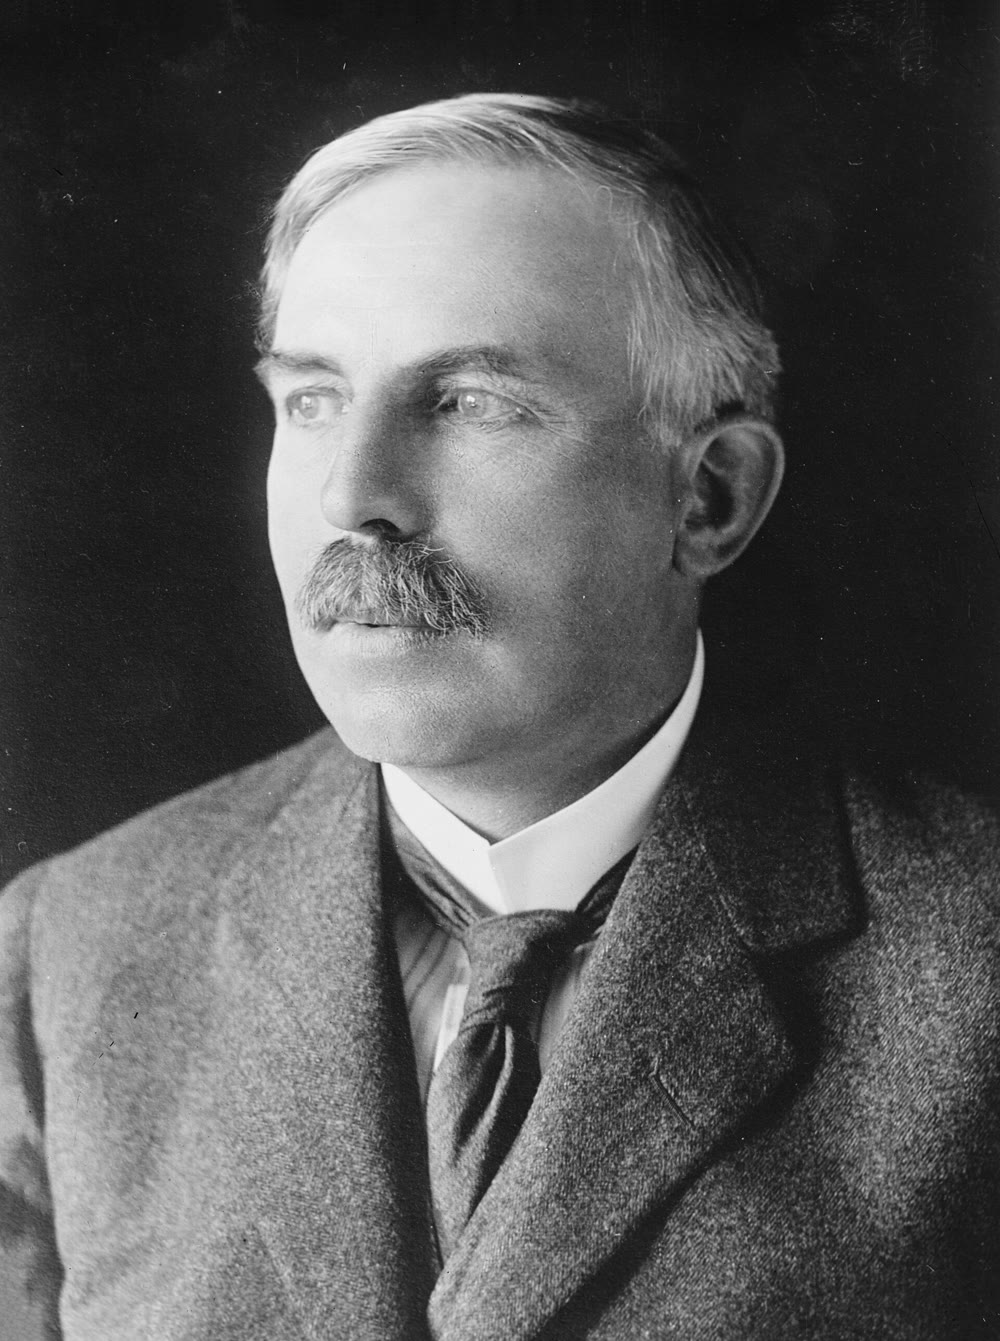
\includegraphics[width=\linewidth]{images/book1/rutherford.jpg}

{\small अर्नेस्ट रदरफ़ोर्ड (1871--1937)।}
\end{minipage}\hfill
\begin{minipage}[b]{0.66\linewidth}\centering
\begin{tikzpicture}[font=\small]
  \fill[black!45] (0,-0.5) rectangle (0.9,0.5);
  \node[anchor=north, align=center] at (0.45,-0.55) {ऐल्फ़ा कणों\\ का स्रोत};
  \draw[->, thick, red!70!black] (0.9,0) -- (2.8,0);
  \fill[yellow!70!orange] (2.8,-1.6) rectangle (2.88,1.6);
  \node[anchor=north] at (2.84,-1.65) {सोने की पत्ती};
  \draw[omDef!40, line width=4pt] (5.6,-1.8) arc[start angle=-30, end angle=30, radius=3.6];
  \foreach \y in {-0.3,-0.1,0.1,0.3} \draw[->, red!70!black] (2.88,\y) -- (5.3,\y);
  \draw[->, red!70!black] (2.88,0.05) -- (5.0,1.15);
  \draw[->, red!70!black] (2.88,-0.05) -- (4.9,-1.3);
  \draw[->, red!70!black, thick] (2.8,0.02) .. controls (2.2,0.35) .. (1.6,0.95);
  \node[anchor=west, align=left, font=\footnotesize] at (6.25,0) {ज़्यादातर\\ सीधे\\ निकल जाते हैं};
  \node[anchor=south, align=center, font=\footnotesize] at (1.6,1.0) {बहुत कम\\ लौट आते हैं};
\end{tikzpicture}

{\small स्वर्ण-पत्र प्रयोग: ज़्यादातर कण सीधे आर-पार निकल जाते हैं; कुछ
विचलित होते हैं; बहुत कम किसी \omterm{def:g9:inside-the-atom:nucleus}{नाभिक} से टकराकर लौट आते हैं।}
\end{minipage}
\end{omfigure}

\section{अभ्यास}

\begin{exercise}[$\star$]\label{exo:g9:inside-the-atom:1}
\omterm{def:g9:inside-the-atom:nucleus}{नाभिक} के कणों और उसके चारों ओर के कणों के नाम, उनके आवेश के चिह्न के
साथ, बताओ।
\end{exercise}

\begin{exercise}[$\star$]\label{exo:g9:inside-the-atom:2}
\ce{^{16}_{8}O}, \ce{^{27}_{13}Al} और \ce{^{40}_{20}Ca} के \omterm{def:g9:inside-the-atom:proton}{प्रोटॉनों},
\omterm{def:g9:inside-the-atom:proton}{न्यूट्रॉनों} और \omterm{def:g9:inside-the-atom:nucleus}{इलेक्ट्रॉनों} की संख्या बताओ।
\end{exercise}

\begin{exercise}[$\star$]\label{exo:g9:inside-the-atom:3}
\omterm{def:g7:atoms-and-molecules:atom}{परमाणु} विद्युत रूप से उदासीन क्यों होता है?
\end{exercise}

\begin{exercise}[$\star$]\label{exo:g9:inside-the-atom:4}
एक \omterm{def:g7:atoms-and-molecules:atom}{परमाणु} में 26 \omterm{def:g9:inside-the-atom:proton}{प्रोटॉन} और 30 \omterm{def:g9:inside-the-atom:proton}{न्यूट्रॉन} हैं। उसका न्यूक्लाइड प्रतीक लिखो
(तत्व लोहा, \ce{Fe}, है)।
\end{exercise}

\begin{exercise}[$\star\star$]\label{exo:g9:inside-the-atom:5}
क्या \ce{^{35}_{17}Cl} और \ce{^{37}_{17}Cl} एक ही तत्व हैं? क्या वे
\omterm{def:g9:inside-the-atom:isotope}{समस्थानिक} हैं? समझाओ।
\end{exercise}

\begin{exercise}[$\star\star$]\label{exo:g9:inside-the-atom:6}
क्या \ce{^{14}_{6}C} और \ce{^{14}_{7}N} \omterm{def:g9:inside-the-atom:isotope}{समस्थानिक} हैं? समझाओ।
\end{exercise}

\begin{exercise}[$\star\star$]\label{exo:g9:inside-the-atom:7}
वैज्ञानिक संकेतन में \ce{^{56}_{26}Fe} के एक \omterm{def:g7:atoms-and-molecules:atom}{परमाणु} का लगभग द्रव्यमान
निकालो।
\end{exercise}

\begin{exercise}[$\star\star$]\label{exo:g9:inside-the-atom:8}
स्वर्ण-पत्र प्रयोग में ज़्यादातर कण सोने के आर-पार सीधे क्यों निकल
जाते हैं?
\end{exercise}

\begin{exercise}[$\star\star$]\label{exo:g9:inside-the-atom:9}
\qty{e-15}{m} का \omterm{def:g9:inside-the-atom:nucleus}{नाभिक} \omterm{def:g7:atoms-and-molecules:atom}{परमाणु} (\qty{e-10}{m}) से कितने गुना छोटा
है? उत्तर दस की घात के रूप में लिखो।
\end{exercise}

\begin{exercise}[$\star\star$]\label{exo:g9:inside-the-atom:10}
किसी तत्व के \omterm{def:g9:inside-the-atom:isotope}{समस्थानिकों} का रसायन एक जैसा क्यों होता है?
\end{exercise}

\begin{exercise}[$\star\star\star$]\label{exo:g9:inside-the-atom:11}
लोहे के एक \omterm{def:g7:atoms-and-molecules:atom}{परमाणु} में 26 \omterm{def:g9:inside-the-atom:nucleus}{इलेक्ट्रॉन} हैं। उनका कुल द्रव्यमान निकालो, फिर
\ce{^{56}_{26}Fe} \omterm{def:g7:atoms-and-molecules:atom}{परमाणु} के द्रव्यमान का वह भिन्न निकालो जो वे बनाते हैं (अभ्यास~7
में निकाले गए द्रव्यमान का उपयोग करो)।
\end{exercise}

\begin{exercise}[$\star\star\star$]\label{exo:g9:inside-the-atom:12}
% ledger: iso:Cu63, iso:Cu65
प्राकृतिक ताँबा \qty{69.15}{\percent} ताँबा-63 और \qty{30.85}{\percent}
ताँबा-65 है। ताँबे के 10\,000 \omterm{def:g7:atoms-and-molecules:atom}{परमाणुओं} में हर \omterm{def:g9:inside-the-atom:isotope}{समस्थानिक} के कितने हैं?
ताँबे के प्रति \omterm{def:g7:atoms-and-molecules:atom}{परमाणु} \omterm{def:g9:inside-the-atom:proton}{न्यूक्लिऑनों} की औसत संख्या कितनी है?
\end{exercise}

\clearpage % keeps the heading with its problem box (it was stranded at a page foot)
\section{समस्या: क्लोरीन को तौलना}

\begin{problem}[{सप्ताहांत समस्या --- क्लोरीन के दो समस्थानिक, हर परमाणु का
द्रव्यमान, और क्लोरीन परमाणु का औसत द्रव्यमान}]
\label{pb:g9:inside-the-atom:1}
% ledger: iso:Cl35, iso:Cl37, const:me, const:mp, const:mn
प्राकृतिक क्लोरीन दो \omterm{def:g9:inside-the-atom:isotope}{समस्थानिकों}, क्लोरीन-35 और क्लोरीन-37, का \omterm{def:g6:pure-substances-and-mixtures:mixture}{मिश्रण} है:
क्लोरीन के 1000 \omterm{def:g7:atoms-and-molecules:atom}{परमाणुओं} में से लगभग 758 क्लोरीन-35 हैं और
242 क्लोरीन-37। एक \omterm{def:g9:inside-the-atom:proton}{न्यूक्लिऑन} का द्रव्यमान \qty{1.67e-27}{kg} और
एक \omterm{def:g9:inside-the-atom:nucleus}{इलेक्ट्रॉन} का द्रव्यमान \qty{9.11e-31}{kg} लो। क्लोरीन का \omterm{def:g9:inside-the-atom:atomic-number}{परमाणु क्रमांक}
17 है।

\medskip
\noindent\textbf{भाग I --- दो \omterm{def:g9:inside-the-atom:nucleus}{नाभिक}।}
\begin{enumerate}
  \item दोनों \omterm{def:g9:inside-the-atom:isotope}{समस्थानिकों} के न्यूक्लाइड प्रतीक लिखो।
  \item हर एक के \omterm{def:g9:inside-the-atom:proton}{प्रोटॉनों}, \omterm{def:g9:inside-the-atom:proton}{न्यूट्रॉनों} और \omterm{def:g9:inside-the-atom:nucleus}{इलेक्ट्रॉनों} की संख्या बताओ।
  \item दोनों को क्लोरीन क्यों कहा जाता है? वे \omterm{def:g9:inside-the-atom:isotope}{समस्थानिक} क्यों हैं?
  \item क्या क्लोरीन-37 का नमूना सोडियम के साथ उसी ढंग से अभिक्रिया करेगा
        जैसे क्लोरीन-35 का नमूना? समझाओ।
\end{enumerate}

\medskip
\noindent\textbf{भाग II --- हर \omterm{def:g7:atoms-and-molecules:atom}{परमाणु} का द्रव्यमान।}
\begin{enumerate}[resume]
  \item क्लोरीन-35 \omterm{def:g7:atoms-and-molecules:atom}{परमाणु} के \omterm{def:g9:inside-the-atom:nucleus}{नाभिक} का द्रव्यमान निकालो।
  \item 17 \omterm{def:g9:inside-the-atom:nucleus}{इलेक्ट्रॉनों} का द्रव्यमान निकालो, और जाँचो कि \omterm{def:g9:inside-the-atom:nucleus}{नाभिक} की तुलना में
        उसे नगण्य माना जा सकता है।
  \item क्लोरीन-37 \omterm{def:g7:atoms-and-molecules:atom}{परमाणु} का द्रव्यमान निकालो।
  \item क्लोरीन-35 के कितने \omterm{def:g7:atoms-and-molecules:atom}{परमाणुओं} का भार \qty{1}{g} होगा? उत्तर
        वैज्ञानिक संकेतन में दो।
\end{enumerate}

\medskip
\noindent\textbf{भाग III --- औसत \omterm{def:g7:atoms-and-molecules:atom}{परमाणु}।}
\begin{enumerate}[resume]
  \item क्लोरीन के कितने प्रतिशत \omterm{def:g7:atoms-and-molecules:atom}{परमाणु} क्लोरीन-35 हैं? क्लोरीन-37?
  \item प्राकृतिक क्लोरीन के 1000 \omterm{def:g7:atoms-and-molecules:atom}{परमाणुओं} में क्लोरीन-35 \omterm{def:g7:atoms-and-molecules:atom}{परमाणुओं} का और
        क्लोरीन-37 \omterm{def:g7:atoms-and-molecules:atom}{परमाणुओं} का कुल द्रव्यमान निकालो।
  \item इन 1000 \omterm{def:g7:atoms-and-molecules:atom}{परमाणुओं} का द्रव्यमान निकालो।
  \item क्लोरीन \omterm{def:g7:atoms-and-molecules:atom}{परमाणु} का औसत द्रव्यमान निकालो।
\end{enumerate}
\end{problem}
